\documentclass{article}
\usepackage[utf8]{inputenc}
\usepackage{hyperref}
\usepackage[letterpaper, portrait, margin=1in]{geometry}
\usepackage{enumitem}
\usepackage{amsmath}
\usepackage{booktabs}
\usepackage{graphicx}

\usepackage{titlesec}

\titleformat{\section}
{\normalfont\Large\bfseries}{\thesection}{1em}{}[{\titlerule[0.8pt]}]
  
\title{Homework 2 Answers}
\author{Economics 7103}
\date{Spring semester 2021}
  
\begin{document}
  
\maketitle

\noindent 1. See table \ref{tab:btable}.  If randomization worked, the simple difference-in-means is an unbiased estimate of the treatment effect.
\begin{table}[h]
    \centering
    \begin{tabular}{llll}
\toprule
{} &   Control & Treatment & Difference \\
{} &    (s.d.) &    (s.d.) &    (p val) \\
\midrule
Electricity  &   1181.33 &   1086.75 &      94.58 \\
             &  (454.31) &  (423.96) &     (0.00) \\
Sqft         &   1633.05 &   1657.55 &     -24.50 \\
             &  (682.90) &  (686.27) &     (0.57) \\
Temp         &     79.89 &     79.89 &      -0.00 \\
             &    (2.16) &    (1.97) &     (0.99) \\
Observations &       501 &       499 &       1000 \\
\bottomrule
\end{tabular}

    \caption{Means by treatment and control group in the sample.  The p value is from a two-way $t$-test for equivalence of means.}
    \label{tab:btable}
\end{table}

\noindent 2. See figure \ref{fig:treatmenthist}, which is non-parametric evidence that the program worked:
\begin{figure}[h]
    \centering
    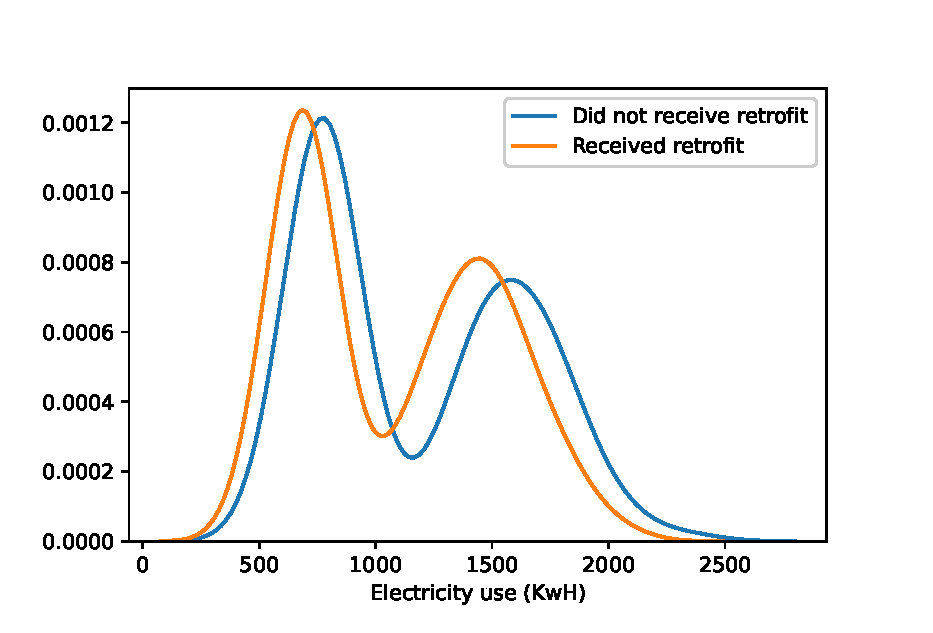
\includegraphics{treatmenthist.eps}
    \caption{Caption}
    \label{fig:treatmenthist}
\end{figure}

\noindent 3. Each method produces quite similar results that probably only differ in rounding error:
\begin{table}[h]
    \centering
   \begin{tabular}{llll}
\toprule
{} &       (a) &       (b) &       (c) \\
\midrule
Retrofit     &  -109.666 &  -109.666 &  -109.666 \\
Sqft         &     0.615 &     0.615 &     0.615 \\
Temperature  &     3.255 &     3.255 &     3.255 \\
Constant     &   -83.603 &   -83.599 &   -83.603 \\
Observations &      1000 &      1000 &      1000 \\
\bottomrule
\end{tabular}

    \caption{Regression coefficients from OLS by hand (a), simulated OLS (b), and using the Statsmodels package (c).}
    \label{tab:outputtable3}
\end{table}
\end{document}